\documentclass[12pt]{article}

\usepackage{discrete}

\def\thetitle{Introduction to Graph Theory} % will be put in the center header on the first page only.
\def\lefthead{Math 228 Notes} % will be put in the left header
\def\righthead{\thetitle} % will be put in the right header



\begin{document}


\section{Coloring}\label{sec:coloring}

\begin{activity}
Mapmakers in the fictional land of Euleria have drawn the borders of the various dukedoms of the land.  To make the map pretty, they wish to color each region.  Adjacent regions must be colored differently, but it is perfectly fine to color two distant regions with the same color.  What is the fewest colors the mapmakers can use and still accomplish this task?

\begin{center}
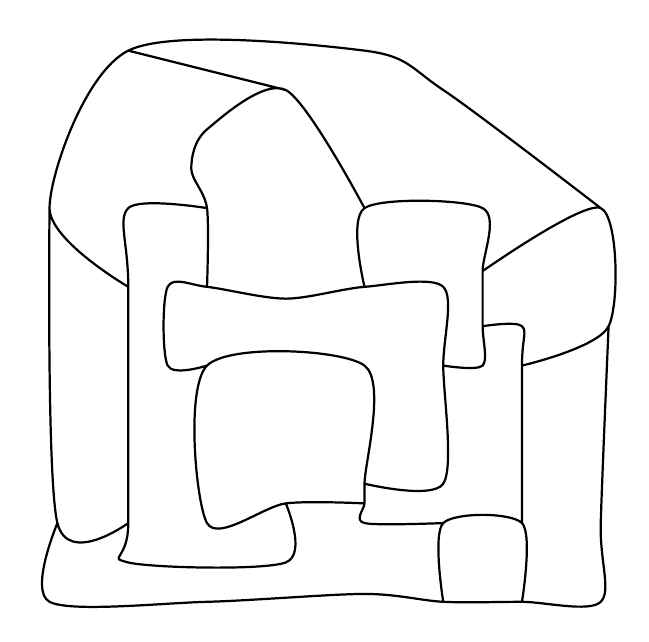
\begin{tikzpicture}
\draw[thick]
	plot [smooth] coordinates {(0.1,1) (0,0) (2,0) (4,0.1) (5,0) (6,0) (7,0) (7,1) (7.1,3.5)}
	plot [smooth] coordinates {(1,1) (0.1,1) (0,5)}
	plot [smooth] coordinates {(2,5) (1,5) (1,4) (1,1) (1,.5) (3,.5) (3,1.25)}
	plot [smooth] coordinates {(5,0) (5,1) (6,1) (6,0)}
	plot [smooth] coordinates {(6,1) (6,3) (6,3.5) (5.5,3.5)}
	plot [smooth] coordinates {(5,1) (4,1) (4,1.25) (4,1.5) (4,3) (2,3) (2,1) (3,1.25) (4,1.25)}
	plot [smooth] coordinates {(4,1.5) (5,1.5) (5,3) (5,4) (4,4) (3,3.85) (2,4) (1.5,4) (1.5,3) (2,3)}
	plot [smooth] coordinates {(5,3) (5.5,3) (5.5,3.5) (5.5, 4.2) (5.5,5) (4,5) (4,4)}
	plot [smooth] coordinates {(6,3) (7.1, 3.5) (7,5) (5.5,4.2)}
	plot [smooth] coordinates {(7,5) (5,6.5) (4,7) (1,7) (0,5) (1,4)}
	plot [smooth] coordinates {(2,4) (2,5) (1.8,5.5) (2,6) (3,6.5) (4,5)}
	plot [smooth] coordinates {(1,7) (3,6.5)};
\end{tikzpicture}
\end{center}

\end{activity}

Perhaps the most famous graph theory problem is how to color maps.

\begin{quote}
 Given any map of countries, states, counties, etc., how many colors are needed to color each region on the map so that neighboring regions are colored differently?
\end{quote}

Actual map makers usually use around seven colors.  For one thing, they require watery regions to be a specific color, and with a lot of colors it is easier to find a permissible coloring.  We want to know whether there is a smaller palette that will work for any map.

How is this related to graph theory?  Well, if we place a vertex in the center of each region (say in the capital of each state) and then connect two vertices if their states share a border, we get a graph.  Coloring regions on the map corresponds to coloring the vertices of the graph.  Since neighboring regions cannot be colored the same, our graph cannot have vertices colored the same when those vertices are adjacent.

In general, given any graph $G$, a coloring of the vertices is called (not surprisingly) a \emph{vertex coloring}\index{vertex coloring}\index{coloring}.  If the vertex coloring has the property that adjacent vertices are colored differently, then the coloring is called \emph{proper}.  Every graph has a proper vertex coloring.  For example, you could color every vertex with a different color.  But often you can do better.  The smallest number of colors needed to get a proper vertex coloring is called the \emph{chromatic number}\index{chromatic number} of the graph, written \gls{chiG}.

\begin{example}
  Find the chromatic number of the graphs below.
  \begin{center}
    \hfill
    \begin{tikzpicture}
      \foreach \x in {0,...,6}
      \draw  (\x*60:1) \v -- (\x*60+60:1) -- (\x*60+180:1) -- cycle;
    \end{tikzpicture}
    \hfill
    \begin{tikzpicture}[yscale=.8]
      \draw  (-1,0) \v -- (0,0) \v -- (1,0) \v -- (.5,1) \v -- (0,0) -- (-.5,1) \v -- (0,2) \v -- (.5,1) -- (-.5,1) -- (-1,0);
    \end{tikzpicture}
    \hfill
    \begin{tikzpicture}[yscale=.8, xscale=1.5]
 \draw  (-1, 0) \v -- (-.5,2) \v -- (0,0) \v -- (.5, 2) \v -- (1,0) \v -- (-.5,2) (.5,2) -- (-1,0);
  \end{tikzpicture}
  \hfill ~
  \end{center}

\begin{solution}
  The graph on the left is $K_6$.  The only way to properly color the graph is to give every vertex a different color (since every vertex is adjacent to every other vertex).  Thus the chromatic number is 6.

  The middle graph can be properly colored with just 3 colors (Red, Blue, and Green).  For example:

  \begin{center}
        \begin{tikzpicture}[yscale=.8]
      \draw  (-1,0) \vb{R} -- (0,0) \vb{B} -- (1,0) \vb{G} -- (.5,1) \vr{R} -- (0,0) -- (-.5,1) \vl{G} -- (0,2) \va{B} -- (.5,1) -- (-.5,1) -- (-1,0);
    \end{tikzpicture}
  \end{center}

  There is no way to color it with just two colors, since there are three vertices mutually adjacent (i.e., a triangle).  Thus the chromatic number is 3.

  The graph on the right is just $K_{2,3}$.  As with all bipartite graphs, this graph has chromatic number 2.   Color the vertices on the top row red and the vertices on the bottom row blue.
\end{solution}

\end{example}

It appears that there is no limit to how large chromatic numbers can get.  It should not come as a surprise that $K_n$ has chromatic number $n$.  So how could there possibly be an answer to the original map coloring question?  If the chromatic number of graph can be arbitrarily large, then it seems like there would be no upper bound to the number of colors needed for any map.  But there is.

The key observation is that while it is true that for any number $n$, there is a graph with chromatic number $n$, only some graphs arrive as representations of maps.  If you convert a map to a graph, the edges between vertices correspond to borders between the countries.  So you should be able to connect vertices in such a way where the edges do not cross.  In other words, the graphs representing maps are all {\em planar}!

So the question is, what is the largest chromatic number of any planar graph?  The answer is one of the best known theorems of mathematics:

\begin{theorem}[The Four Color Theorem\index{Four Color Theorem}]
If $G$ is a planar graph, then the chromatic number of $G$ is less than or equal to 4.  Thus any map can be properly colored with 4 or fewer colors.
\end{theorem}

We will not prove this theorem.  Really.  Even though the theorem is easy to state and understand, the proof is not.  In fact, there is currently no ``easy'' known proof of the theorem.  The current best proof still requires powerful computers to check an {\em unavoidable set} of  633 {\em reducible configurations}.  The idea is that every graph must contain one of these reducible configurations (this fact also needs to be checked by a computer) and that reducible configurations can, in fact, be colored in 4 or fewer colors.


\subsection{Coloring in General}
\begin{activity}
The math department plans to offer 10 classes next semester.  Some classes cannot run at the same time (perhaps they are taught by the same professor, or are required for seniors).

\begin{center}
\begin{tabular}{cl}
\textbf{Class:} & \textbf{Conflicts with:} \\ \hline
A & D I \\
B & D I J \\
C & E F I \\
D & A B F \\
E & H I\\
F & I\\
G & J \\
H & E I J\\
I & A B C E F H \\
J & B G H
\end{tabular}
\end{center}

How many different time slots are needed to teach these classes (and which should be taught at the same time)?  More importantly, how could we use graph coloring to answer this question?
\end{activity}


Cartography is certainly not the only application of graph coloring.  There are plenty of situations in which you might wish partition the objects in question so that related objects are not in the same set.  For example, you might wish to store chemicals safely.  To avoid explosions, certain pairs of chemicals should not be stored in the same room.  By coloring a graph (with vertices representing chemicals and edges representing potential negative interactions), you can determine the smallest number of rooms needed to store the chemicals.

Here is a further example:

\begin{example}
Radio stations broadcast their signal at certain frequencies.  However, there are a limited number of frequencies to choose from, so nationwide many stations use the same frequency.  This works because the stations are far enough apart that their signals will not interfere; no one radio could pick them up at the same time.

Suppose 10 new radio stations are to be set up in a currently unpopulated (by radio stations) region.  The radio stations that are close enough to each other to cause interference are recorded in the table below.  What is the fewest number of frequencies the stations could use.

\centerline{\begin{tabular}{c|c|c|c|c|c|c|c|c|c|c|}
 & {\tiny KQEA}&{\tiny KQEB}&{\tiny KQEC}&{\tiny KQED}&{\tiny KQEE}&{\tiny KQEF}&{\tiny KQEG}&{\tiny  KQEH}&{\tiny  KQEI}&{\tiny KQEJ } \\ \hline
{\tiny KQEA }&      &      &   x  &      &      &   x  &   x  &      &      &  x   \\ \hline
{\tiny KQEB }&      &      &   x  &   x  &      &      &      &      &      &      \\ \hline
{\tiny KQEC }&   x  &      &      &      &      &   x  &   x  &      &      &  x   \\ \hline
{\tiny KQED }&      &  x   &      &      &  x   &  x   &      &  x   &      &      \\ \hline
{\tiny KQEE }&      &      &      &  x   &      &      &      &      &  x   &      \\ \hline
{\tiny KQEF }&  x   &      &  x   &  x   &      &      &   x  &      &      &  x   \\ \hline
{\tiny KQEG }&  x   &      &  x   &      &      &  x   &      &      &      &  x   \\ \hline
{\tiny KQEH }&      &      &      &  x   &      &      &      &      &  x   &      \\ \hline
{\tiny KQEI }&      &      &      &      &  x   &      &      &  x   &      &  x   \\ \hline
{\tiny KQEJ }&  x   &      &  x   &      &      &  x   &   x  &      &  x   &      \\ \hline
\end{tabular}}

\begin{solution}
Represent the problem as a graph with vertices as the stations and edges when two stations are close enough to cause interference.  We are looking for the chromatic number of the graph.  Vertices that are colored identically represent stations that can have the same frequency.

This graph has chromatic number 5.  A proper 5-coloring is shown on the right.  Notice that the graph contains a copy of the complete graph $K_5$ so no fewer than 5 colors can be used.

\begin{center}
\begin{tikzpicture}[scale=.9]
\coordinate (A) at (90:2);
\coordinate (B) at (90-36:2);
\coordinate (C) at (90-2*36:2);
\coordinate (D) at (90-3*36:2);
\coordinate (E) at (90-4*36:2);
\coordinate (F) at (90-5*36:2);
\coordinate (G) at (90-6*36:2);
\coordinate (H) at (90-7*36:2);
\coordinate (I) at (90-8*36:2);
\coordinate (J) at (90-9*36:2);

\draw (A) -- (F) -- (D) -- (H) -- (I) (G) -- (J) -- (C) -- (F) (C) -- (G) -- (A) -- (J);

\draw (A) \va{\tiny KQEA} -- (C) \vr{\tiny KQEC} -- (B) \va{\tiny KQEB} -- (D) \vr{\tiny KQED} -- (E) \vb{\tiny KQEE} -- (I) \vl{\tiny KQEI} -- (J) \va{\tiny KQEJ} -- (F) \vb{\tiny KQEF} -- (G) \vl{\tiny KQEG} (H) \vl{\tiny KQEH};
\end{tikzpicture}
\qquad \qquad
\begin{tikzpicture}[scale=.9]
\coordinate (A) at (90:2);
\coordinate (B) at (90-36:2);
\coordinate (C) at (90-2*36:2);
\coordinate (D) at (90-3*36:2);
\coordinate (E) at (90-4*36:2);
\coordinate (F) at (90-5*36:2);
\coordinate (G) at (90-6*36:2);
\coordinate (H) at (90-7*36:2);
\coordinate (I) at (90-8*36:2);
\coordinate (J) at (90-9*36:2);

\draw (A) -- (F) -- (D) -- (H) -- (I) (G) -- (J) -- (C) -- (F) (C) -- (G) -- (A) -- (J);
\draw[line width=1.25pt] (A) -- (C) -- (F) -- (G) -- (J) -- (A) -- (F) -- (J) -- (C) -- (G) -- (A);

\draw (A) \va{\tiny R} -- (C) \vr{\tiny B} -- (B) \va{\tiny G} -- (D) \vr{\tiny B} -- (E) \vb{\tiny G} -- (I) \vl{\tiny B} -- (J) \va{\tiny P} -- (F) \vb{\tiny G} -- (G) \vl{\tiny Y} (H) \vl{\tiny R};
\end{tikzpicture}

\end{center}

\end{solution}
\end{example}

%\begin{example}
%Your high school chemistry teacher is getting a new lab.  She will need cabinets to store various chemicals.  To avoid explosions, it is important that some pairs of chemicals are definitely not stored in the same cabinet.   What is the fewest number of cabinets the chemist can use to store these chemicals?
%
%\begin{solution}
%
%\end{solution}
%\end{example}

In the example above, the chromatic number was 5, but this is not a counterexample to the Four Color Theorem, since the graph representing the radio stations is not planar.  It would be nice to have some quick way to find the chromatic number of a (possibly non-planar) graph.  It turns out nobody knows whether an efficient algorithm for computing chromatic numbers exists.

While we might not be able to find the exact chromatic number of graph easily, we can often give a reasonable range for the chromatic number.  In other words, we can give upper and lower bounds for chromatic number.

This is actually not very difficult: for every graph $G$, the chromatic number of $G$ is at least 1 and at most the number of vertices of $G$.

What?  You want \emph{better} bounds on the chromatic number?  Well you are in luck.

A \emph{clique}\index{clique} in a graph is a set of vertices all of which are pairwise adjacent.  In other words, a clique of size $n$ is just a copy of the complete graph $K_n$.  We define the \emph{clique number} of a graph to be the largest $n$ for which the graph contains a clique of size $n$.  Any clique of size $n$ cannot be colored with fewer than $n$ colors, so we have a nice lower bound:

\begin{theorem}
The chromatic number of a graph $G$ is at least the clique number of $G$.
\end{theorem}

There are times when the chromatic number of $G$ is \emph{equal} to the clique number.  These graphs have a special name -- they are called \emph{perfect}\index{perfect graph}.  If you know that a graph is perfect, then finding the chromatic number is simply a matter of searching for the largest clique.\footnote{There are special classes of graphs which can be proved to be perfect.  One such class is the set of \emph{chordal} graphs, which have the property that every cycle in the graph contains a \emph{chord} -- an edge between two vertices in of the cycle which are not adjacent in the cycle.}  However, not all graphs are perfect.

For an upper bound, we can improve on ``the number of vertices'' by looking to the degrees of vertices.  Let \gls{deltaG} be the largest degree of any vertex in the graph $G$.  One reasonable guess for an upper bound on the chromatic number is $\chi(G) \le \Delta(G) + 1$.  Why is this reasonable?  Starting with any vertex, it together with all of its neighbors can always be colored in $\Delta(G) + 1$ colors, since at most we are talking about $\Delta(G) + 1$ vertices in this set.  Now fan out!  At any point, if you consider an already colored vertex, some of its neighbors might be colored, some might not.  But no matter what, that vertex and its neighbors could all be colored distinctly, since there are at most $\Delta(G)$ neighbors, plus the one vertex being considered.

In fact, there are examples of graphs for which $\chi(G) = \Delta(G) + 1$.  For any $n$, the complete graph $K_n$ has chromatic number $n$, but $\Delta(K_n) = n-1$ (since every vertex is adjacent to every \emph{other} vertex).  Additionally, any \emph{odd} cycle will have chromatic number 3, but the degree of every vertex in a cycle is 2.  It turns out that these are the only two types of examples where we get equality, a result known as Brooks' Theorem.

\begin{theorem}[Brooks' Theorem\index{Brooks' Theorem}]
Any graph $G$ with maximal degree $\Delta(G)$ satisfies $\chi(G) \le \Delta(G)$, unless $G$ is a complete graph or an odd cycle, in which case $\chi(G) = \Delta(G) + 1$.
\end{theorem}

The proof of this theorem is \emph{just} complicated enough that we will not present it here (although you are asked to prove a special case in the exercises).  The adventurous reader is encouraged to find a book on graph theory for suggestions on how to prove the theorem.



%\begin{activity}
%A \emph{proper vertex coloring} of a graph is a coloring in which no two adjacent vertices are colored the same color.  The \emph{chromatic number} of a graph is the smallest number of colors needed for a proper coloring of the graph.
%
%For each graph below, find a proper coloring and determine the chromatic number of the graph.  As you are working on these colorings, think about the following ideas:
%\begin{enumerate}
%\item Before I even start coloring the graph, can I come up with an upper bound on the number of colors I will need (a bound that is better than simply the total number of vertices in the graph)?
%
%\item Before I even start coloring the graph, can I come up with a lower bound on the number of colors I will need (a bound that is better than simply 2)?
%
%\item Once you have colored the graph, make sure that you check your coloring with your tablemates to try to determine if you used the minimal number of colors.  Talk with each other about reasons why you couldn't have used fewer colors than you did.
%
%\item For each graph, try to identify if it is a type of graph that we've talked about before (i.e.\ does it have a special name or special properties).  If the graph is a named graph, try to see if you can generalize the ideas you used in your coloring of this graph to other graphs of that same type.
%\end{enumerate}
%
%ADD GRAPHS!
%
%\end{activity}\todo{Replace this with a map coloring question}



\subsection{Coloring Edges}


The chromatic number of a graph tells us about coloring vertices, but we could also ask about coloring edges.  Just like with vertex coloring, we might insist that edges that are adjacent must be colored differently.  Here, we are thinking of two edges as being adjacent if they are incident to the same vertex.  The least number of colors required to properly color the edges of a graph $G$ is called the \emph{chromatic index}\index{chromatic index} of $G$, written \gls{chiindG}.

\begin{example}
Six friends decide to spend the afternoon playing chess.  Everyone will play everyone else once.  They have plenty of chess sets but nobody wants to play more than one game at a time.  Games will last an hour (thanks to their handy chess clocks).  How many hours will the tournament last?

\begin{solution}
Represent each player with a vertex and put an edge between two players if they will play each other.  In this case, we get the graph $K_6$:

\begin{center}
\begin{tikzpicture}
\foreach \x in {0,...,5}{

	\foreach \y in {1,...,5}{
	 \draw (\x*60:1) -- (\x*60+\y*60:1);
	}
\draw (\x*60:1) \v;
}
\end{tikzpicture}
\end{center}

We must color the edges; each color represents a different hour.  Since different edges incident to the same vertex will be colored differently, no player will be playing two different games (edges) at the same time.  Thus we need to know the chromatic index of $K_6$.

Notice that for sure $\chi'(K_6) \ge 5$, since there is a vertex of degree 5. It turns out 5 colors is enough (go find such a coloring).  Therefore the friends will play for 5 hours.
\end{solution}
\end{example}

Interestingly, if one of the friends in the above example left, the remaining 5 chess-letes would still need 5 hours: the chromatic index of $K_5$ is also 5.

In general, what can we say about chromatic index?  Certainly $\chi'(G) \ge \Delta(G)$.  But how much higher could it be?  Only a little higher.

\begin{theorem}[Vizing's Theorem\index{Vizing's Theorem}]
For any graph $G$, the chromatic index $\chi'(G)$ is either $\Delta(G)$ or $\Delta(G) + 1$.
\end{theorem}

At first this theorem makes it seem like chromatic index might not be very interesting.  However, deciding which case a graph is in is not always easy.  Graphs for which $\chi'(G) = \Delta(G)$ are called \emph{class 1}, while the others are called \emph{class 2}. Bipartite graphs always satisfy $\chi'(G) = \Delta(G)$, so are class 1 (this was proved by K\"onig in 1916, decades before Vizing proved his theorem in 1964).  In 1965 Vizing proved that all planar graphs with $\Delta(G) \ge 8$ are of class 1, but this does not hold for all planar graphs with $2 \le \Delta(G) \le 5$.  Vizing conjectured that all planar graphs with $\Delta(G) = 6$ or $\Delta(G) = 7$ are class 1; the $\Delta(G) = 7$ case was proved in 2001 by Sanders and Zhao; the $\Delta(G) = 6$ case is still open.


There is another interesting way we might consider coloring edges, quite different from what we have discussed so far.  What if we colored every edge of a graph either red or blue.  Can we do so without, say, creating a \emph{monochromatic}\index{monochromatic} triangle (i.e., an all red or all blue triangle)?  Certainly for some graphs the answer is yes. Try doing so for $K_4$.  What about $K_5$?  $K_6$?  How far can we go?

The answer to the above problem is known and is a fun problem to do as an exercise.  We could extend the question in a variety of ways.  What if we had three colors?  What if we were trying to avoid other graphs.  The surprising fact is that very little is known about these questions.  For example, we know that you need to go up to $K_{17}$ in order to force a monochromatic triangle using three colors, but nobody knows how big you need to go with more colors.  Similarly, we know that using two colors $K_{18}$ is the smallest graph that forces a monochromatic copy of $K_4$, but the best we have to force a monochromatic $K_{5}$ is a range, somewhere from $K_{43}$ to $K_{49}$.  If you are interested in these sorts of questions, this area of graph theory is called Ramsey theory\index{Ramsey theory}.  Check it out.


\end{document}
